\documentclass[../../../../dd.tex]{subfiles}

\begin{document}

	\section{Deployment View}
		
		The main hardware devices involved in this system are the following:
		\begin{itemize} 
		\item Web Server: on this server there is the logic tier of the application, this tier contains the logical part of the system, so this devices must have the higher computation power between the devices. It offers via HTTP the connection from the user, and accesses to the database via XMPP ( communication protocol based on XML typical used for inter-server communication).
		\item Data Base Server: on this server there is the data tier of the application. This device must store in its memory all the data of the system. So, to avoid problem, the memory of this device must be suitable to store all the information. This device must be connected to the web server with the purpose of making available to the logic tier the information that the data tier store. The communication between these two tiers takes place in XMPP.
		\item User Devices: this kind of devices is divided into Mobile Devices and Computers. In this kind of devices there is the presentation tier of the application. The kind of component used on this devices depends on the type of devices and on the OS installed (as we have described on the chapter Software Limitation in the RASD) . We can't know the hardware specification of this devices, so the presentation tier must be as light as possible. The communication between these devices and the Web Server takes place in HTTP through the internet.
	\end{itemize}
	
	
	\begin{figure}[H]
				\centering
				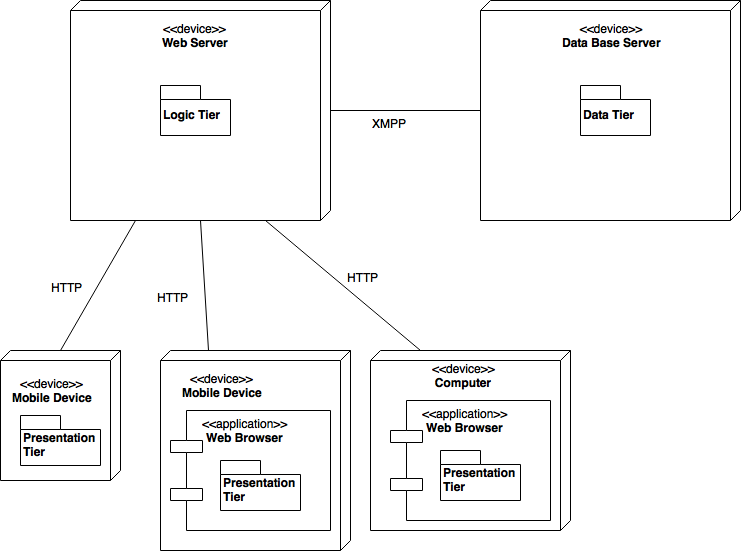
\includegraphics[width=\textwidth, scale=0.5]{../images/Deploy.png}
			\caption{Deployment Diagram}\label{fig:Deploy}
		\end{figure}
	
\end{document}